% DSO138 user manual. Compile with pdfLaTeX twice; no external images required.
\documentclass[10pt,a4paper]{article}
\usepackage[T1]{fontenc}
\usepackage[utf8]{inputenc}
\usepackage{lmodern}
\renewcommand{\familydefault}{\sfdefault}
\usepackage[a4paper,left=18mm,right=18mm,top=17mm,bottom=16mm,
  includeheadfoot,headheight=14pt,headsep=6mm,footskip=9mm]{geometry}
\usepackage{microtype}
\usepackage[table]{xcolor}
\usepackage{graphicx}
\usepackage{tikz}
\usetikzlibrary{arrows.meta,calc,positioning}
\usepackage{booktabs,tabularx,array}
\usepackage{enumitem}
\usepackage{amsmath}
\usepackage{tcolorbox}
\usepackage{titlesec,fancyhdr,lastpage}
\usepackage{hyperref}
\definecolor{navy}{HTML}{172B4D}
\definecolor{teal}{HTML}{006F80}
\definecolor{ink}{HTML}{25334A}
\definecolor{muted}{HTML}{5B677A}
\definecolor{line}{HTML}{CBD5E1}
\definecolor{pale}{HTML}{EDF6F7}
\definecolor{orange}{HTML}{D87B2E}
\definecolor{trace}{HTML}{FFE15C}
\hypersetup{pdftitle={DSO138 Oscilloscope User Manual},
  pdfauthor={DSO138 Firmware Project},
  pdfsubject={Operating guide for DSO138 unreleased firmware source revision},
  colorlinks=true,linkcolor=teal,urlcolor=teal,bookmarksopen=true}
\setlength{\parindent}{0pt}
\setlength{\parskip}{5pt}
\setlength{\emergencystretch}{2em}
\setlength{\tabcolsep}{5pt}
\renewcommand{\arraystretch}{1.15}
\setlist{leftmargin=*,itemsep=3pt,topsep=3pt,parsep=0pt}
\setlist[enumerate]{label=\textcolor{teal}{\bfseries\arabic*.}}
\setlist[itemize]{label=\textcolor{teal}{\textbullet}}
\titleformat{\section}{\color{navy}\Large\bfseries}{\thesection}{0.65em}{}
\titlespacing*{\section}{0pt}{0pt}{10pt}
\titleformat{\subsection}{\color{teal}\normalsize\bfseries}{}{0pt}{}
\titlespacing*{\subsection}{0pt}{9pt}{3pt}
\pagestyle{fancy}
\fancyhf{}
\fancyhead[L]{\small\bfseries\color{navy}DSO138}
\fancyhead[R]{\small\color{muted}USER MANUAL}
\fancyfoot[L]{\footnotesize\color{muted}Manual 1.2 \enspace|\enspace Firmware: unreleased revision}
\fancyfoot[R]{\footnotesize\color{muted}\thepage\,/\,\pageref*{LastPage}}
\renewcommand{\headrulewidth}{0.4pt}
\renewcommand{\footrulewidth}{0pt}
\newcommand{\key}[1]{\mbox{\fcolorbox{line}{white}{\strut\footnotesize\bfseries #1}}}
\newcommand{\lcd}[1]{\texttt{#1}}
\newcommand{\manualpage}[2]{\clearpage\section{#1}\label{#2}}
\newtcolorbox{manualnote}[1]{colback=pale,colframe=teal,boxrule=0pt,
  leftrule=2pt,arc=0pt,left=8pt,right=8pt,
  top=6pt,bottom=6pt,title={#1},fonttitle=\bfseries\small,
  coltitle=teal,colbacktitle=pale,toptitle=5pt,bottomtitle=0pt,
  before skip=7pt,after skip=7pt}
\newcolumntype{Y}{>{\raggedright\arraybackslash}X}
\newcommand{\coverlink}[2]{\hyperref[#1]{#2}\hfill
  {\color{muted}\pageref*{#1}}}
\newcommand{\screenfigure}{%
  \begin{center}
  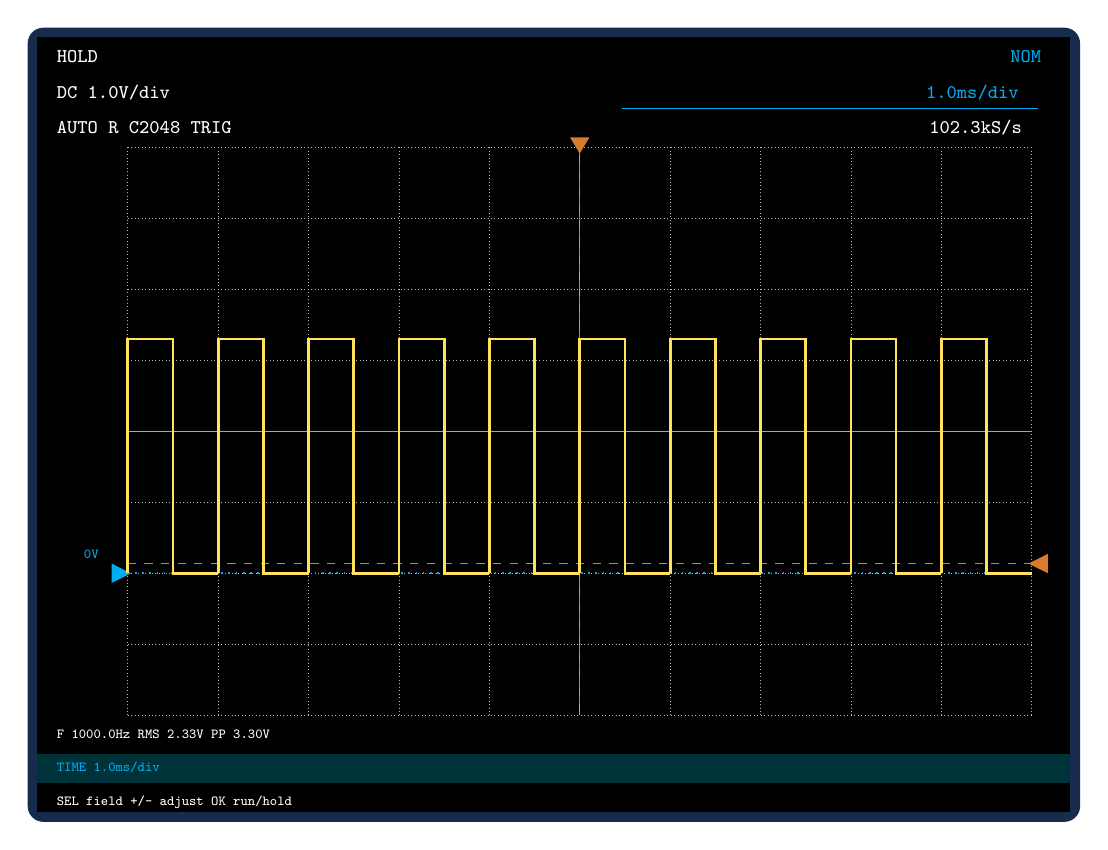
\begin{tikzpicture}[x=0.41mm,y=-0.41mm,font=\sffamily]
    \fill[navy,rounded corners=2mm] (-3,-3) rectangle (323,243);
    \fill[black] (0,0) rectangle (320,240);
    \node[anchor=west,text=white,font=\ttfamily\scriptsize] at (3,6) {HOLD};
    \node[anchor=east,text=cyan,font=\ttfamily\scriptsize] at (314,6) {NOM};
    \node[anchor=west,text=white,font=\ttfamily\scriptsize] at (3,17) {DC 1.0V/div};
    \node[anchor=east,text=cyan,font=\ttfamily\scriptsize] at (307,17) {1.0ms/div};
    \draw[cyan,line width=0.6pt] (181,22)--(310,22);
    \node[anchor=west,text=white,font=\ttfamily\scriptsize] at (3,28) {AUTO R C2048 TRIG};
    \node[anchor=east,text=white,font=\ttfamily\scriptsize] at (308,28) {102.3kS/s};
    \foreach \xx in {28,56,...,308}{\draw[gray!55,densely dotted,line width=0.25pt] (\xx,34)--(\xx,210);}
    \foreach \yy in {34,56,...,210}{\draw[gray!55,densely dotted,line width=0.25pt] (28,\yy)--(308,\yy);}
    \draw[gray!70,line width=0.4pt] (28,122)--(308,122) (168,34)--(168,210);
    \draw[orange,dashed,line width=0.5pt] (168,34)--(168,210);
    \draw[orange,dashed,line width=0.5pt] (28,163)--(308,163);
    \fill[orange] (165,31)--(171,31)--(168,36)--cycle;
    \fill[orange] (313,160)--(307,163)--(313,166)--cycle;
    \draw[cyan,dotted,line width=0.6pt] (28,166)--(308,166);
    \fill[cyan] (23,163)--(29,166)--(23,169)--cycle;
    \node[anchor=east,text=cyan,font=\ttfamily\tiny] at (22,160) {0V};
    \foreach \start in {28,56,...,280}{
      \draw[trace,line width=1pt] (\start,166)--(\start,93.4)
        --++(14,0)--++(0,72.6)--++(14,0);
    }
    \node[anchor=west,text=white,font=\ttfamily\tiny] at (3,216) {F 1000.0Hz RMS 2.33V PP 3.30V};
    \fill[teal!45!black] (0,222) rectangle (320,231);
    \node[anchor=west,text=cyan,font=\ttfamily\tiny] at (3,226) {TIME 1.0ms/div};
    \node[anchor=west,text=white,font=\ttfamily\tiny] at (3,237) {SEL field  +/- adjust  OK run/hold};
  \end{tikzpicture}

  {\footnotesize\color{muted}Illustrative layout, not a screenshot or a measured record.}
  \end{center}}
\begin{document}
\fontsize{10.3pt}{13.5pt}\selectfont
\thispagestyle{empty}
\vspace*{1mm}
{\color{teal}\rule{24mm}{2mm}}\par
\vspace{6mm}
{\fontsize{54}{57}\selectfont\bfseries\color{navy}DSO138}\par
{\fontsize{27}{32}\selectfont\bfseries\color{navy}Oscilloscope}\par
\vspace{2mm}
{\fontsize{22}{27}\selectfont\color{teal}User manual}\par
\vspace{4mm}
{\large Classic board \enspace|\enspace C++ firmware}\par
\vspace{7mm}
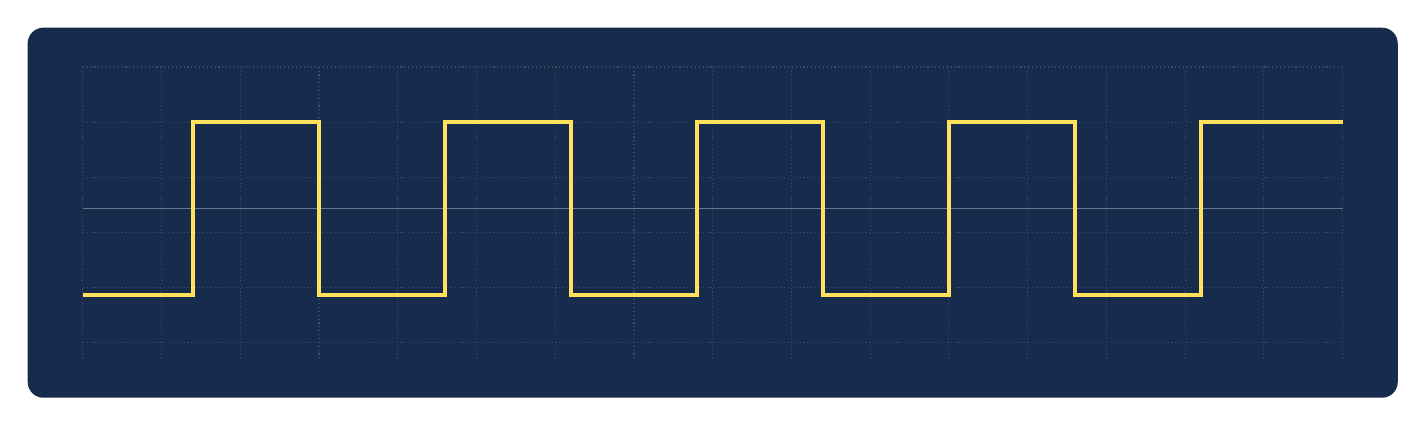
\begin{tikzpicture}[x=1mm,y=1mm]
  \fill[navy,rounded corners=2mm] (0,0) rectangle (174,47);
  \foreach \xx in {7,17,...,167}{\draw[white!16!navy,densely dotted] (\xx,5)--(\xx,42);}
  \foreach \yy in {7,14,...,42}{\draw[white!16!navy,densely dotted] (7,\yy)--(167,\yy);}
  \draw[white!35!navy] (7,24)--(167,24);
  \draw[trace,line width=1.5pt] (7,13)--(21,13)--(21,35)--(37,35)--(37,13)
    --(53,13)--(53,35)--(69,35)--(69,13)--(85,13)--(85,35)
    --(101,35)--(101,13)--(117,13)--(117,35)--(133,35)--(133,13)
    --(149,13)--(149,35)--(167,35);
\end{tikzpicture}
\vspace{3mm}
\begin{tabularx}{\linewidth}{@{}YYY@{}}
  {\Large\bfseries\color{teal}4 keys} &
  {\Large\bfseries\color{teal}9 ranges} &
  {\Large\bfseries\color{teal}24 timebases}\\
  Run, hold and edit & 10\,mV/div to 5\,V/div &
  10\,$\mu$s/div to 500\,s/div
\end{tabularx}
\vspace{6mm}
{\color{navy}\large\bfseries Find what you need}\par
\begin{minipage}[t]{0.47\linewidth}
  \coverlink{quickstart}{First measurement}\par
  \coverlink{controls}{Physical controls}\par
  \coverlink{screen}{Reading the screen}\par
  \coverlink{menu}{Complete menu map}\par
  \coverlink{triggering}{Triggering and held records}\par
  \coverlink{measurements}{Measurements}\par
\end{minipage}\hfill
\begin{minipage}[t]{0.47\linewidth}
  \coverlink{slow}{Slow signals and rolling}\par
  \coverlink{storage}{Save, recall and settings}\par
  \coverlink{calibration}{Optional DC calibration}\par
  \coverlink{troubleshooting}{Troubleshooting}\par
  \coverlink{reference}{Reference and scope}\par
\end{minipage}
\vfill
{\small\color{muted}
Manual revision 1.2 \enspace|\enspace 1 November 2026\par
Firmware source: unreleased revision (UID-configured build required)\par
Intended hardware: PCB 109-13800-00C, STM32F103C8T6, ILI9341 display.\par
This guide describes the implemented controls and functions.
Nominal readings are not a calibration certificate.}

\manualpage{Quick start}{quickstart}

\begin{manualnote}{Board and power}
This guide is for the identified DSO138 board, PCB 109-13800-00C, with STM32F103C8T6 and ILI9341 display. Use the board's normal 9 V DC input as marked on the board. For bench work, use a low-voltage isolated supply and connect signal ground to the scope ground. Use only isolated low-voltage bench signals; never connect the scope input or ground directly to mains. Do not infer a safe maximum input from this guide; observe the board markings and its analog input limits.
\end{manualnote}

This operating guide assumes a correctly configured firmware image. The current unreleased source revision requires each owner to set the MCU UID and board identity before normal startup; see the repository's Getting started guide.

\subsection*{Try the built-in signal}
\begin{enumerate}
\item Connect the onboard test output to the signal input.
\item Set the physical coupling switch to DC, base sensitivity to 1 V/div, and multiplier to \(\times1\).
\item Press \key{SEL} until Timebase is selected. Use \key{+}/\key{-} to select 1 ms/div.
\item Select Trigger mode and choose AUTO with \key{+}/\key{-}.
\item In an ordinary field such as Timebase, press \key{OK} if the scope is in HOLD. Look for RUN and a repeating square wave.
\item Press \key{OK} again to hold the record for inspection.
\end{enumerate}
The observed board showed about 3.3 vertical divisions and a frequency near 1 kHz in this setup. This is a functional check, not a guaranteed voltage, frequency standard, or calibration reference.

On power-up, saved valid settings return in HOLD; press \key{OK} to run. If there are no saved settings, the enabled board profile requests Auto run after the physical switches settle. Waveform recall is always a separate, explicit action. Allow the display to show a record before judging a signal.

\textbf{The three slide switches set the analog input.} Their positions physically select coupling and sensitivity. Software settings cannot move them. After changing a switch, wait for the on-screen status to leave \lcd{WAIT INPUT} or \lcd{Switches settling} before using a new record.

\manualpage{Buttons and physical switches}{controls}

\begin{tabularx}{\linewidth}{@{}p{0.16\linewidth}X@{}}
\toprule
Control & Action \\
\midrule
\key{SEL} & Move to the next setting field. After Calibration, the sequence returns to Timebase. \\
\key{+}, \key{-} & Change a value or cycle a choice. For numeric settings, holding a button repeats after about 400 ms, then at about 80 ms intervals. Discrete choices do not repeat. \\
\key{OK} & Run or hold in ordinary fields; rearm Single when appropriate. In Storage or Calibration, the first press stops acquisition and a later press executes the selected action. Release between presses. \\
\key{RESET} & Hardware reset. Unsaved edits are lost; the last saved configuration normally returns in HOLD. A reset during flash erase/program can lose saved data; see Saving. \\
\bottomrule
\end{tabularx}

The controls accept one button action at a time. If buttons are pressed together, release them before trying again. A completed Single capture or a fault may need an acknowledgement before the next action; wait for the status to settle, release, then press \key{OK} again when the screen indicates the action is ready.

\begin{tabularx}{\linewidth}{@{}p{0.27\linewidth}XXX@{}}
\toprule
Base sensitivity & Multiplier \(\times1\) & Multiplier \(\times2\) & Multiplier \(\times5\) \\
\midrule
10 mV/div & 10 mV/div & 20 mV/div & 50 mV/div \\
100 mV/div & 100 mV/div & 200 mV/div & 500 mV/div \\
1 V/div & 1 V/div & 2 V/div & 5 V/div \\
\bottomrule
\end{tabularx}

The separate coupling switch selects DC, AC, or GND.

The table gives the nine nominal ranges. The separate coupling switch selects DC (shows the input offset), AC (blocks DC), or GND (selects the internal ground path). These are front-panel sensitivity labels. They do not confirm the input voltage or a probe's attenuation. If using a \(\times10\) probe, account for that factor yourself; there is no probe-attenuation menu.

\subsection*{Trigger activity LED}
D3 gives a brief, about 100 ms indication for an accepted trigger crossing; another crossing restarts the pulse, so close events may look continuously lit. Auto free-run timeout, recall/HOLD redraw and slow Auto ROLL do not light it. On slow Normal or Single, an accepted edge may light it before the processed record is ready. A Single pulse can finish through automatic HOLD; faults leave it off. This software cue is not a precise timing strobe and has not been tested on hardware.

\manualpage{Reading the screen}{screen}

\screenfigure

The display status tells you what the instrument is doing: \lcd{RUN} or \lcd{ARM} indicates active acquisition or arming, \lcd{HOLD} indicates a stopped view, and \lcd{WAIT INPUT} or \lcd{WAIT BACK} means it is waiting for stable switches or an acquisition backend. On slow settings you may see \lcd{WARMUP}, \lcd{ROLL}, or \lcd{WAIT TRIG}; see Slow timebases.

The plot has 10 horizontal and 8 vertical divisions. The yellow trace/envelope shows available samples; drawing does not create extra samples. Orange marks the trigger position and level; cyan marks the zero reference and selected control. Focus labels beginning \lcd{NEXT} show the value to be used by the next capture, while a held trace continues to show its frozen capture settings. The reference line is labeled \lcd{0V} with a usable voltage profile, or \lcd{REF} when values are raw ADC codes.

The top labels show coupling, sensitivity, timebase, trigger mode/edge/level and sample spacing or rate. A held waveform keeps the range, coupling, timing and calibration provenance from its capture. If a slide switch changes, the old held trace is not rescaled to the new analog setting; the display may say \lcd{OLD range/coupling held}. Start a fresh capture to inspect the new setting.

\textbf{Reading the grid:} 3.3 vertical divisions at 1 V/div represent about 3.3 V peak-to-peak. One full cycle spanning one horizontal division at 1 ms/div represents a 1 ms period, or about 1 kHz. Apply an external probe's attenuation factor separately.

The quality tag describes voltage conversion: \lcd{NOM} uses nominal board coefficients, \lcd{CAL} means a measured profile is installed, and \lcd{RAW} means no voltage conversion is available. None of these labels by itself certifies measurement accuracy. Clipping warnings mean amplitude and frequency results are invalid for that record.

\manualpage{Menu and settings}{menu}

Press \key{SEL} to move through the twelve fields. Use \key{+} and \key{-} to adjust; use \key{OK} as shown. The focused field is shown near the bottom of the screen.

\begin{tabularx}{\linewidth}{@{}p{0.25\linewidth}p{0.40\linewidth}X@{}}
\toprule
Focus & \(+\)/\(-\) & \key{OK} \\
\midrule
Timebase & Select a catalogue setting & Run/Hold \\
Trigger mode & AUTO, NORMAL, SINGLE & Run/Hold; Single rearm \\
Trigger edge & Rising or falling & Run/Hold; Single rearm \\
Trigger level & ADC threshold, 16-code steps & Run/Hold; Single rearm \\
Trigger position & 0--100\%, 2.5\% steps & Run/Hold; Single rearm \\
Vertical position & Move reference, 2-pixel steps & Run/Hold; Single rearm \\
Horizontal position & Pan, 16-sample steps & Run/Hold; Single rearm \\
Measurements & Overview, Amplitude, RMS/Mean, Freq & Run/Hold \\
Storage & Choose one of six actions & Stop, then execute \\
Calibration reference & Set signed reference value & Stop, then cycle step \\
Calibration tolerance & Set allowed error & Stop, then cycle step \\
Calibration & Begin, Accept Ref, Install, Abort & Stop, then execute \\
\bottomrule
\end{tabularx}

For Storage and Calibration, if acquisition is running, the first \key{OK} changes to HOLD. Release the button, then press \key{OK} again to carry out the selected action. In Reference and Tolerance, \key{OK} in HOLD cycles the decimal edit step; \key{+} and \key{-} change the value by that step. Use \lcd{SAVE CONFIG} for the eight scope settings listed under Storage. Reference/tolerance editors are not saved by that action.

\manualpage{Triggering and viewing}{triggering}

\begin{itemize}[leftmargin=*]
\item \textbf{AUTO:} publishes a record when a trigger edge qualifies, or after its timeout if no qualifying edge arrives. Use it for a general live view and for the built-in signal check.
\item \textbf{NORMAL:} waits for the selected edge at the trigger level. If the signal never crosses the level in the selected direction, it can keep waiting.
\item \textbf{SINGLE:} captures one complete record and stops. Press \key{OK} to arm another capture. If the completed record or a fault has not yet been acknowledged, wait for the screen state, release, and press again.
\end{itemize}

Choose rising or falling edge in Trigger edge. Trigger level changes in 16 ADC-code steps; it is a code threshold, not a calibrated voltage setting. Trigger position moves from 0\% to 100\% of the record in 2.5\% steps, selecting how much history lies before the trigger in ordinary triggered captures.

Timebase, trigger mode, edge, level and trigger position affect capture. Changing them during a run invalidates the incomplete record. On a held or recalled trace, timebase changes zoom the existing samples; they do not resample the waveform. Areas outside the captured record remain empty. Vertical \key{+} moves the reference down; \key{-} moves it up. Horizontal \key{+} pans toward later source samples; \key{-} pans toward earlier samples, in 16-sample steps. These view adjustments do not make a new capture.

\subsection*{Example: trigger position at 50\%}
\begin{center}
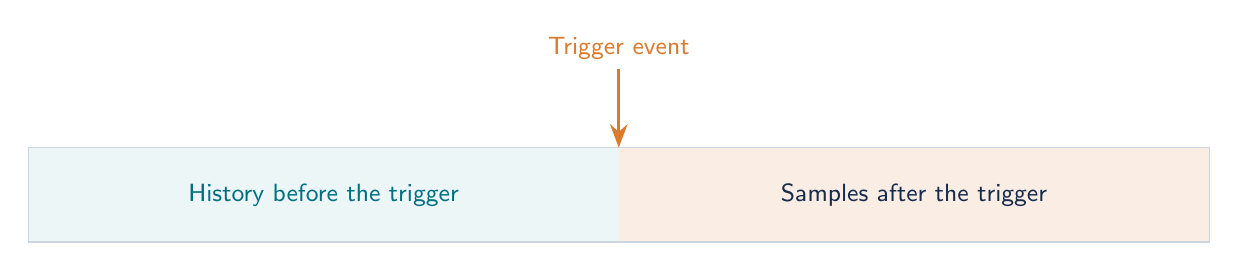
\begin{tikzpicture}[x=1mm,y=1mm,font=\small]
  \fill[pale] (0,0) rectangle (75,12);
  \fill[orange!13] (75,0) rectangle (150,12);
  \draw[line] (0,0) rectangle (150,12);
  \node[teal] at (37.5,6) {History before the trigger};
  \node[navy] at (112.5,6) {Samples after the trigger};
  \draw[orange,very thick,-{Stealth}] (75,22)--(75,12);
  \node[above,text=orange] at (75,22) {Trigger event};
\end{tikzpicture}

{\footnotesize\color{muted}Record position before any view pan or timebase zoom.}
\end{center}

Use HOLD to inspect a stable record, then RUN to resume. With AC coupling, the instrument cannot show the DC component removed by the input circuit. With GND coupling, the trace shows the grounded input path, not an external signal.

\manualpage{Measurements and validity}{measurements}

Measurements cover the complete finite record, not just the visible portion or a hand-selected cycle. The four measurement pages are Overview, Amplitude, RMS/Mean and Freq.

\begin{tabularx}{\linewidth}{@{}p{0.25\linewidth}X@{}}
\toprule
Screen item & Meaning \\
\midrule
MIN, MAX & Lowest and highest sampled values in the record. \\
PP & Peak-to-peak, the difference between maximum and minimum. \\
PK & Peak magnitude from the voltage zero; it is not necessarily half of PP when a DC offset is present. \\
RMS & Total RMS about the calibration zero, including DC. \\
AC, AC-RMS & RMS after subtracting the record mean. \\
MEAN, AVG & Arithmetic mean of the record. \\
F & Detected repetition rate, when valid. \\
\bottomrule
\end{tabularx}

With \lcd{RAW}, the display reports ADC codes (marked \lcd{c}) rather than input volts. \lcd{NOM} uses the board's nominal conversion coefficients. \lcd{CAL} means an installed measured DC profile is being used. A displayed voltage is a converted estimate, not an accuracy guarantee. AC-coupled mean and total RMS describe the AC-coupled signal; they cannot restore removed DC.

Frequency needs at least three qualified complete periods. A clear trace can still show \lcd{-- CYCLES} when it is too short. Other reasons can include low amplitude, instability, clipping, grounding or a rate outside estimator limits. Frequency is observed repetition, not proof of the signal's fundamental frequency. Aliasing can produce a plausible but incorrect value.

Any ADC rail hit or slow-filter clamp suppresses valid amplitude and frequency claims; the display may show \lcd{ADC CLIP}, \lcd{RAW ADC CLIP}, \lcd{FIR CLAMP}, or \lcd{F -- CLIP; volts invalid}. A missing voltage profile gives \lcd{RAW: no volts}. Stop and correct the input/range before relying on another record. As a mathematical illustration only, an ideal 0-to-3.3 V, 50\% duty square wave has 3.3 V PP, 1.65 V mean, 2.33 V total RMS and 1.65 V AC RMS. These calculated values are not a test or specification of the onboard output.

\manualpage{Slow timebases}{slow}

The six slow settings use rolling history. A full 10-division window takes a long time to fill. The first valid filtered point appears after the nominal warm-up shown here; the delay is additional history behind the point being displayed.

\begin{tabularx}{\linewidth}{@{}p{0.18\linewidth}p{0.24\linewidth}p{0.24\linewidth}X@{}}
\toprule
Setting & 10-division span & First valid point & Nominal output rate \\
\midrule
10 s/div & 100 s & 2.9 s & 5.12 samples/s \\
20 s/div & 200 s & 5.8 s & 2.56 samples/s \\
50 s/div & 500 s & 14.6 s & 1.024 samples/s \\
100 s/div & 1,000 s & 29.1 s & 0.512 samples/s \\
200 s/div & 2,000 s & 58.3 s & 0.256 samples/s \\
500 s/div & 5,000 s & 145.7 s & 0.1024 samples/s \\
\bottomrule
\end{tabularx}

The active filtered mode takes 25 raw ADC samples for each output interval and applies two digital filter stages. The first valid output appears after about 14.92 output intervals of warm-up; the filter's delay is about 7.44 output intervals. Wait through \lcd{WARMUP} before judging the trace. These timing values describe the configured design, not a measured accuracy or noise specification. Slow settings are useful for observing slow changes and drift; do not infer that a rapidly changing signal is captured between the sparse output points.

\begin{itemize}[leftmargin=*]
\item \lcd{ROLL} means Auto is building/updating rolling history.
\item \lcd{WAIT TRIG} means Normal or Single is waiting for a qualifying trigger.
\item \lcd{AA25} marks the filtered path. Its digital filter does not prevent aliasing of signals above the raw ADC Nyquist limit; use suitable external signal bandwidth limits.
\end{itemize}

Use DC coupling for slow levels or drift: AC coupling can suppress very slow changes. Slow-mode analog response is not fully physically qualified. Faster screen redraw cannot replace missing samples.

\manualpage{Saving, loading and recalling}{storage}

Storage offers six actions in the Storage field. Select one with \key{+}/\key{-}; waveform saving requires a complete, fully processed held record. A valid recalled record may also be saved. If running, press \key{OK}, release, then press it again to execute. Wait for \lcd{SAVED} after a save before changing power or resetting.

\begin{tabularx}{\linewidth}{@{}p{0.27\linewidth}X@{}}
\toprule
Displayed action & What it does \\
\midrule
\lcd{SAVE WAVE} & Store the latest complete waveform and current eight scope settings in the single waveform slot, with captured timing, physical and calibration metadata. \\
\lcd{RECALL WAVE} & Restore the saved settings and record together as a held view. Recall is explicit; it does not install its calibration into the live bank. \\
\lcd{SAVE CONFIG} & Save the eight scope settings (timebase, trigger mode/edge/level/position, vertical/horizontal position and measurement page). It preserves the waveform slot. \\
\lcd{LOAD CONFIG} & Restore saved UI settings. The restored settings start in HOLD. \\
\lcd{SAVE CAL} & Persist the currently installed calibration bank. \\
\lcd{RESTORE CAL} & Restore the saved calibration bank into the live profile. A valid calibration bank is also restored at boot. \\
\bottomrule
\end{tabularx}

To save a trace: obtain a complete record, press \key{OK} to HOLD if necessary, select \lcd{SAVE WAVE}, then execute with a fresh \key{OK}. This stores the waveform and its current scope settings together. To recall: select \lcd{RECALL WAVE} in HOLD and execute; the saved record and settings return together in HOLD. To save settings alone without replacing the waveform slot, select \lcd{SAVE CONFIG}. Reference and tolerance editor values are not part of the eight saved scope settings; calibration persistence is separate through \lcd{SAVE CAL}.

\begin{manualnote}{Single-bank flash warning}
Saved records occupy one 2\,KiB storage region in the device flash. A reset or power loss during flash erase/program can lose the waveform, settings or calibration. Do not interrupt a save; wait for \lcd{SAVED}. Completed \lcd{SAVE CONFIG} and \lcd{SAVE CAL} operations normally preserve the waveform; \lcd{SAVE WAVE} replaces it. The lower-bank area used by older firmware now holds the application, and migration of older saved data is not guaranteed.
\end{manualnote}

Flash endurance is finite. Avoid repeated unnecessary saves. Physical interruption recovery and endurance have not been fully qualified. \lcd{HOLD TO SAVE} means first obtain and hold a complete processed record. A recalled waveform cannot be used as an applied calibration reference.

\manualpage{Optional DC calibration}{calibration}

Leave the nominal profile in place unless you have suitable, stable reference-voltage equipment. The onboard test output is not a calibration standard. Calibration converts ADC codes to voltage for DC measurements; it does not qualify AC response, bandwidth, the clock or probe attenuation.

The procedure uses two DC references to fit a profile and a separate third DC reference to check it. Each must be a fresh held live record with unchanged physical switch settings, at least 64 samples, spread no greater than 32 ADC codes, and no rail samples. The two fitting records must differ by at least 64 ADC codes. The third must lie at least 16 codes inside both fitted endpoints and pass the selected tolerance. A reference value is entered for each record. Enter values in microvolts (\(\mu\mathrm{V}\)): \(1{,}000{,}000\,\mu\mathrm{V}=1\,\mathrm{V}\). These editor values are not input ratings.

To acquire each reference, leave the calibration fields with \key{SEL}, select an ordinary field such as Timebase, then use \key{OK} for RUN and HOLD. \key{OK} inside a calibration field never starts acquisition.

\begin{enumerate}[leftmargin=*]
\item Set DC coupling and one fixed range. In HOLD, choose \lcd{BEGIN} and execute. Apply reference 1, set its known value in Calibration reference, RUN and acquire, then HOLD and choose \lcd{ACCEPT REF}.
\item Apply a different reference 2. Update Calibration reference to its known value, acquire a fresh record, HOLD, then choose \lcd{ACCEPT REF} again.
\item Apply independent reference 3. Update Calibration reference to its known value and set Calibration tolerance to the allowed error. Acquire a fresh record, HOLD, and choose \lcd{ACCEPT REF}. The session should show \lcd{VERIFIED}.
\item Choose \lcd{INSTALL} and execute. The profile is now installed in RAM for the matching DC range. To keep it across restart, select \lcd{SAVE CAL} in Storage and execute separately.
\item Choose \lcd{ABORT} to discard a pending candidate. Abort leaves any already installed profile in place.
\end{enumerate}

In Reference and Tolerance, \key{OK} cycles the decimal step (powers of ten); it does not move a cursor digit by digit. \key{+}/\key{-} changes the numeric value by that step. Replace an unsuitable held record with a fresh one. A switch change, failed two-point fit or failed third-point check requires \lcd{BEGIN} and a new session. Installation and saving do not certify hardware accuracy; an external comparison is still required.

\manualpage{Troubleshooting}{troubleshooting}

\begin{tabularx}{\linewidth}{@{}p{0.34\linewidth}X@{}}
\toprule
Screen status or symptom & What to do \\
\midrule
No trace or an empty plot & Choose AUTO, return to RUN and wait for a record. Set vertical and horizontal position to zero; a panned or zoomed held view can lie outside the captured data. \\
\lcd{WAIT INPUT}, \lcd{Switches settling} & Check the physical slide-switch positions and allow them to settle. \\
\lcd{WAIT BACK}, \lcd{No slow capture; view only} & The selected timebase/backend is unavailable in this run. Choose a supported timebase or restart the instrument if the condition persists. \\
\lcd{WARMUP} & Wait for the slow filter to produce its first valid output. \\
\lcd{WAIT TRIG} & In Normal or Single, check that the input crosses the selected trigger level and edge. \\
\lcd{-- CYCLES} & Select a wider time span so more periods fit in the fixed record. For the onboard signal, try 1 ms/div. \\
\lcd{RAW: no volts} & Voltage calibration is unavailable. Read ADC codes only or restore/use an appropriate profile. \\
\lcd{ADC CLIP}, \lcd{FIR CLAMP} & Reduce the input or choose a suitable physical range, then capture again. \\
\lcd{OLD range/coupling held} & The held record belongs to the previous switch setting. Run a fresh capture. \\
\lcd{HOLD TO SAVE} & Wait in HOLD for a complete, fully processed record, then retry. \\
\lcd{EMPTY}, \lcd{READ ONLY}, \lcd{DISABLED} & The requested storage item is absent or the action is unavailable; check selection and status. \\
\lcd{ERROR}, \lcd{Save failed; kept; OK retry} & The previous record remains held when available. Wait, then retry once with a fresh \key{OK}; if it repeats, stop using storage and restart normally. \\
\lcd{FAULT} & Wait for the fault state, release all buttons, then use a fresh \key{OK} retry if offered. \\
\bottomrule
\end{tabularx}

If a button appears ignored, press only one at a time and release it fully before the next action. In Storage or Calibration, remember that the first \key{OK} may only stop acquisition. Use a second press after release to execute. Do not reset during a save.

\manualpage{Reference and scope}{reference}

\textbf{Timebase catalogue} (time per horizontal division):\par\smallskip
\begin{tabularx}{\linewidth}{@{}p{0.25\linewidth}X@{}}
\toprule
Unit & Values \\
\midrule
Microseconds (\(\mu\)s/div) & 10, 20, 50, 100, 200, 500 \\
Milliseconds (ms/div) & 1, 2, 5, 10, 20, 50, 100, 200, 500 \\
Seconds (s/div) & 1, 2, 5, 10, 20, 50, 100, 200, 500 \\
\bottomrule
\end{tabularx}

There are 24 settings. Fast acquisition uses a configured maximum of 500 ksample/s; this is a timer plan, not an independently measured sample rate, jitter or timebase accuracy. Slow settings use the rolling path described earlier. The horizontal scale, display refresh and acquisition rate are different quantities.

\textbf{Voltage and probe limits.} Nominal range labels and \lcd{NOM} conversion use board coefficients; they are not a production calibration. \lcd{CAL} indicates a measured profile is installed, but does not replace independent verification. \lcd{RAW} provides codes, not input volts. No probe attenuation is selected by firmware; multiply displayed input estimates by the probe factor when applicable. Do not treat the onboard signal as an absolute reference. No maximum safe input is specified here: follow the board's own input markings and limits.

\begin{manualnote}{Firmware identity and qualification}
The operating and qualification observations in this manual refer to the previously deployed b73 firmware image on the identified board profile, with nominal gain-2 coefficients and a grounded-zero code; its reported build image SHA-256 begins \texttt{b73cdcb1c644}. Public firmware source release 1.0.1 adds the trigger activity LED described under Controls. Its LED pulse, acquisition handoff and startup/fault sequencing passed software checks; 1.0.1 has not been flashed or tested on hardware. The current unreleased source revision changes saved-data layout to a single flash bank as described under Saving; it has not been flashed or tested on hardware. This change does not complete physical production qualification. Independent voltage, frequency, bandwidth, loaded timing, slow-path performance and long-term storage qualification remain open. Use the instrument as a functional oscilloscope with these limits in mind, not as a calibrated laboratory instrument.
\end{manualnote}

\vfill
\begin{center}\footnotesize Manual revision 1.2: 1 November 2026. Operator reference sources: \texttt{firmware/App/Src/dso\_ui\_model.cpp}, \texttt{firmware/App/Src/dso\_ui\_controller.cpp}, \texttt{firmware/App/Src/dso\_scaling.cpp}, and \texttt{firmware/App/Inc/dso\_timebase\_presets.hpp}.\end{center}


\end{document}
